%---------------
%╔═╗╔═╗╔╦╗╦  ╦╔═╗
%╚═╗║╣    ║  ║  ║╠═╝
%╚═╝╚═╝  ╩  ╚═╝╩  
%---------------

% language setup
\newcommand{\docLanguage}{ngerman}
%\newcommand{\docLanguage}{english}

% DOCUMENT SETUP
\documentclass[12pt, oneside, a4paper, \docLanguage]{report}
\usepackage[left=3cm, 
			right=2.5cm, 
			top=2.5cm, 
			bottom=2.5cm, 
			includehead, 
			includefoot]{geometry}

% line spacing
\usepackage{setspace}
\setstretch{1,25} % 15/12 --> 1.25

% encoding setup
% T1 font encoding for languages that use a latin alphabet
\usepackage[T1]{fontenc} 

% enhanced input encoding handling - utf8 for äÄüÜöÖß...
\usepackage[utf8]{inputenc}

%de­fines Adobe Times Ro­man as de­fault text font
\usepackage{mathptmx}
\usepackage{times} % needed for acronym package

%PDF linking package
\usepackage[hidelinks]{hyperref}


% Language Setup
\usepackage[\docLanguage]{babel}
% after babel - set chapter string
\AtBeginDocument{\renewcommand{\chaptername}{}}

% language specific bibliography style
\usepackage[numbers, square]{natbib}
%\setcitestyle{square,aysep={},yysep={;}}
\usepackage[fixlanguage]{babelbib}
\selectbiblanguage{\docLanguage}
% bliographystyle setup
% babel specific: babplain, babplai3, babalpha, babunsrt, bababbrv, bababbr3
\bibliographystyle{babunsrt}


% enumeration
\usepackage{enumitem}
% tabular extension tabularx
\usepackage{tabularx}

% math packages
\usepackage{amsmath}
\usepackage{nicefrac}
\usepackage{amsthm}
\usepackage{amsbsy}
\usepackage{amssymb}
\usepackage{amsfonts}
%\usepackage{MnSymbol}


%special characters
\usepackage{amssymb}
\usepackage{upgreek,textgreek}

% acronym package
\usepackage[printonlyused, footnote]{acronym}

% breakable text in \seqsplit{}
\usepackage{seqsplit}

% \textmu
\usepackage{textcomp}

% package provides a way to compile sections of a document using the same preamble as the main document
\usepackage{subfiles}

% driver-independent color extension - used by listings,tabularx
\usepackage[usenames,dvipsnames,table,xcdraw]{xcolor}

% -- SYNTAX HIGHLIGHTING --
\usepackage{listings}
%% bash command line Syntax Highlighting
\lstdefinestyle{BASH_CMD}{ 
  columns=fullflexible,            % copy pasteable listings
  language=bash,
  basicstyle=\small\sffamily,
  basicstyle   = \small \ttfamily,
  keywordstyle = [1]\small \ttfamily,
  keywordstyle = [2]\small \ttfamily,
  commentstyle = \small \ttfamily,
  numbers=none,
  captionpos=b, 
  breaklines=true,
  numberstyle=\tiny,
  numbersep=3pt,
  frame=tlrb,
  columns=fullflexible,
  backgroundcolor=\color{white!20},
  linewidth=\linewidth,
  literate=                        % replace in code
     {Ö}{{\"O}}1 
     {Ä}{{\"A}}1 
     {Ü}{{\"U}}1 
     {ß}{{\ss}}2 
     {ü}{{\"u}}1 
     {ä}{{\"a}}1 
     {ö}{{\"o}}1 
     {â}{{\^{a}}}1 
     {Â}{{\^{A}}}1 
     {ç}{{\c{c}}}1 
     {Ç}{{\c{C}}}1 
     {ğ}{{\u{g}}}1 
     {Ğ}{{\u{G}}}1 
     {ı}{{\i}}1 
     {İ}{{\.{I}}}1 
     {ş}{{\c{s}}}1 
     {Ş}{{\c{S}}}1 
}
 % adds style BASH_CMD
%% Matlab Syntax Highlighting
\colorlet{keyword}{blue!100!black!80}
\colorlet{STD}{Lavender}
\colorlet{comment}{green!90!black!90}
\definecolor{mygreen}{rgb}{0,0.6,0}
\definecolor{mygray}{rgb}{0.5,0.5,0.5}
\definecolor{mymauve}{rgb}{0.58,0,0.82}


\lstdefinestyle{BASH_SCRIPT}{ 
  language     = bash,
  basicstyle   = \footnotesize \ttfamily,
  keywordstyle = [1]\color{keyword}\bfseries,
  keywordstyle = [2]\color{STD}\bfseries,
  commentstyle = \color{mygreen}\itshape,
  backgroundcolor=\color{white},   % choose the background color; you must add \usepackage{color} 
  columns=fullflexible,            % copy pasteable listings
                                   % or \usepackage{xcolor}
  basicstyle=\footnotesize,        % the size of the fonts that are used for the code
  breakatwhitespace=false,         % sets if automatic breaks should only happen at whitespace
  breaklines=true,                 % sets automatic line breaking
  captionpos=b,                    % sets the caption-position to bottom
  extendedchars=true,              % lets you use non-ASCII characters; for 8-bits encodings only,
                                   % does not work with UTF-8
  frame=single,                    % adds a frame around the code
  keepspaces=true,                 % keeps spaces in text, useful for keeping indentation of code
                                   % (possibly needs columns=flexible)
  numbers=left,                    % where to put the line-numbers; possible values are 
                                   % (none, left, right)
  numbersep=5pt,                   % how far the line-numbers are from the code
  numberstyle=\tiny\color{mygray}, % the style that is used for the line-numbers
  rulecolor=\color{black},         % if not set, the frame-color may be changed on line-breaks
                                   % within not-black text (e.g. comments (green here))
  showspaces=false,                % show spaces everywhere adding particular underscores; it
  	                               % overrides 'showstringspaces'
  showstringspaces=false,          % underline spaces within strings only
  showtabs=false,                  % show tabs within strings adding particular underscores
  stepnumber=1,                    % the step between two line-numbers. If it's 1, each line 
                                   % will be numbered
  stringstyle=\color{mymauve},     % string literal style
  tabsize=2,                       % sets default tabsize to 2 spaces
  title=\lstname,                  % set title name
  literate=                        % replace in code
     {Ö}{{\"O}}1 
     {Ä}{{\"A}}1 
     {Ü}{{\"U}}1 
     {ß}{{\ss}}2 
     {ü}{{\"u}}1 
     {ä}{{\"a}}1 
     {ö}{{\"o}}1 
     {â}{{\^{a}}}1 
     {Â}{{\^{A}}}1 
     {ç}{{\c{c}}}1 
     {Ç}{{\c{C}}}1 
     {ğ}{{\u{g}}}1 
     {Ğ}{{\u{G}}}1 
     {ı}{{\i}}1 
     {İ}{{\.{I}}}1 
     {ş}{{\c{s}}}1 
     {Ş}{{\c{S}}}1 
} % adds style BASH_SCRIPT
% Matlab Syntax Highlighting
\colorlet{keyword}{blue!100!black!80}
\colorlet{STD}{red}
\colorlet{comment}{green!90!black!90}
\definecolor{mygreen}{rgb}{0,0.6,0}
\definecolor{mygray}{rgb}{0.5,0.5,0.5}
\definecolor{mymauve}{rgb}{0.58,0,0.82}


\lstdefinestyle{LATEX}{ 
  language     = [LaTeX]{TeX},
  basicstyle   = \footnotesize \ttfamily,
  keywordstyle = [1]\color{keyword}\bfseries,
  keywordstyle = [2]\color{comment}\bfseries,
  commentstyle = \color{mygray}\itshape,
  %backgroundcolor=\color{white},   % choose the background color; you must add \usepackage{color} 
                                   % or \usepackage{xcolor}
  basicstyle=\footnotesize,        		   % the size of the fonts that are used for the code
  breakatwhitespace=false,         % sets if automatic breaks should only happen at whitespace
  columns=fullflexible,            % copy pasteable listings
  breaklines=true,                 % sets automatic line breaking
  captionpos=c,                    % sets the caption-position to bottom
  extendedchars=true,              % lets you use non-ASCII characters; for 8-bits encodings only,
                                   % does not work with UTF-8
  frame=single,                    % adds a frame around the code
  keepspaces=true,                 % keeps spaces in text, useful for keeping indentation of code
                                   % (possibly needs columns=flexible)
  numbers=left,                    % where to put the line-numbers; possible values are 
                                   % (none, left, right)
  numbersep=4pt,                   % how far the line-numbers are from the code
  numberstyle=\tiny\color{mygray}, % the style that is used for the line-numbers
  rulecolor=\color{black},         % if not set, the frame-color may be changed on line-breaks
                                   % within not-black text (e.g. comments (green here))
  showspaces=false,                % show spaces everywhere adding particular underscores; it
  	                               % overrides 'showstringspaces'
  showstringspaces=false,          % underline spaces within strings only
  showtabs=false,                  % show tabs within strings adding particular underscores
  stepnumber=1,                    % the step between two line-numbers. If it's 1, each line 
                                   % will be numbered
  stringstyle=\color{mymauve},     % string literal style
  tabsize=2,                       % sets default tabsize to 2 spaces
  title=\lstname,                  % set title name
  literate=                        % replace in code
     {Ö}{{\"O}}1 
     {Ä}{{\"A}}1 
     {Ü}{{\"U}}1 
     {ß}{{\ss}}2 
     {ü}{{\"u}}1 
     {ä}{{\"a}}1 
     {ö}{{\"o}}1 
     {â}{{\^{a}}}1 
     {Â}{{\^{A}}}1 
     {ç}{{\c{c}}}1 
     {Ç}{{\c{C}}}1 
     {ğ}{{\u{g}}}1 
     {Ğ}{{\u{G}}}1 
     {ı}{{\i}}1 
     {İ}{{\.{I}}}1 
     {ş}{{\c{s}}}1 
     {Ş}{{\c{S}}}1 
} % adds style LATEX
%% Matlab Syntax Highlighting
\colorlet{keyword}{blue!100!black!80}
\colorlet{STD}{Lavender}
\colorlet{comment}{green!90!black!90}
\definecolor{mygreen}{rgb}{0,0.6,0}
\definecolor{mygray}{rgb}{0.5,0.5,0.5}
\definecolor{mymauve}{rgb}{0.58,0,0.82}


\lstdefinestyle{MATLAB}{ 
  language     = Matlab,
  basicstyle   = \footnotesize \ttfamily,
  keywordstyle = [1]\color{keyword}\bfseries,
  keywordstyle = [2]\color{STD}\bfseries,
  commentstyle = \color{mygreen}\itshape,
  backgroundcolor=\color{white},   % choose the background color; you must add \usepackage{color} 
                                   % or \usepackage{xcolor}
  basicstyle=\footnotesize,        % the size of the fonts that are used for the code
  breakatwhitespace=false,         % sets if automatic breaks should only happen at whitespace
  columns=fullflexible,            % copy pasteable listings
  breaklines=false,                % sets automatic line breaking
  captionpos=c,                    % sets the caption-position to bottom
  extendedchars=true,              % lets you use non-ASCII characters; for 8-bits encodings only,
                                   % does not work with UTF-8
  frame=single,                    % adds a frame around the code
  keepspaces=true,                 % keeps spaces in text, useful for keeping indentation of code
                                   % (possibly needs columns=flexible)
  numbers=left,                    % where to put the line-numbers; possible values are 
                                   % (none, left, right)
  numbersep=5pt,                   % how far the line-numbers are from the code
  numberstyle=\tiny\color{mygray}, % the style that is used for the line-numbers
  rulecolor=\color{black},         % if not set, the frame-color may be changed on line-breaks
                                   % within not-black text (e.g. comments (green here))
  showspaces=false,                % show spaces everywhere adding particular underscores; it
  	                               % overrides 'showstringspaces'
  showstringspaces=false,          % underline spaces within strings only
  showtabs=false,                  % show tabs within strings adding particular underscores
  stepnumber=1,                    % the step between two line-numbers. If it's 1, each line 
                                   % will be numbered
  stringstyle=\color{mymauve},     % string literal style
  tabsize=2,                       % sets default tabsize to 2 spaces
  title=\lstname,                  % set title name
  literate=                        % replace in code
     {Ö}{{\"O}}1 
     {Ä}{{\"A}}1 
     {Ü}{{\"U}}1 
     {ß}{{\ss}}2 
     {ü}{{\"u}}1 
     {ä}{{\"a}}1 
     {ö}{{\"o}}1 
     {â}{{\^{a}}}1 
     {Â}{{\^{A}}}1 
     {ç}{{\c{c}}}1 
     {Ç}{{\c{C}}}1 
     {ğ}{{\u{g}}}1 
     {Ğ}{{\u{G}}}1 
     {ı}{{\i}}1 
     {İ}{{\.{I}}}1 
     {ş}{{\c{s}}}1 
     {Ş}{{\c{S}}}1 
} % adds style MATLAB
% Matlab Syntax Highlighting
\colorlet{keyword}{blue!100!black!80}
\colorlet{STD}{Lavender}
\colorlet{comment}{green!90!black!90}
\definecolor{mygreen}{rgb}{0,0.6,0}
\definecolor{mygray}{rgb}{0.5,0.5,0.5}
\definecolor{mymauve}{rgb}{0.58,0,0.82}


\lstdefinestyle{PYTHON}{ 
  language     = Python,
  basicstyle   = \footnotesize \ttfamily,
  keywordstyle = [1]\color{keyword}\bfseries,
  keywordstyle = [2]\color{STD}\bfseries,
  commentstyle = \color{mygreen}\itshape,
  backgroundcolor=\color{white},   % choose the background color; you must add \usepackage{color} 
                                   % or \usepackage{xcolor}
  basicstyle=\footnotesize,        % the size of the fonts that are used for the code
  columns=fullflexible,            % copy pasteable listings
  breakatwhitespace=false,         % sets if automatic breaks should only happen at whitespace
  breaklines=false,                % sets automatic line breaking
  captionpos=c,                    % sets the caption-position to bottom
  extendedchars=true,              % lets you use non-ASCII characters; for 8-bits encodings only,
                                   % does not work with UTF-8
  frame=single,                    % adds a frame around the code
  keepspaces=true,                 % keeps spaces in text, useful for keeping indentation of code
                                   % (possibly needs columns=flexible)
  numbers=left,                    % where to put the line-numbers; possible values are 
                                   % (none, left, right)
  numbersep=5pt,                   % how far the line-numbers are from the code
  numberstyle=\tiny\color{mygray}, % the style that is used for the line-numbers
  rulecolor=\color{black},         % if not set, the frame-color may be changed on line-breaks
                                   % within not-black text (e.g. comments (green here))
  showspaces=false,                % show spaces everywhere adding particular underscores; it
  	                               % overrides 'showstringspaces'
  showstringspaces=false,          % underline spaces within strings only
  showtabs=false,                  % show tabs within strings adding particular underscores
  stepnumber=1,                    % the step between two line-numbers. If it's 1, each line 
                                   % will be numbered
  stringstyle=\color{mymauve},     % string literal style
  tabsize=2,                       % sets default tabsize to 2 spaces
  title=\lstname,                  % set title name
  literate=                        % replace in code
     {Ö}{{\"O}}1 
     {Ä}{{\"A}}1 
     {Ü}{{\"U}}1 
     {ß}{{\ss}}2 
     {ü}{{\"u}}1 
     {ä}{{\"a}}1 
     {ö}{{\"o}}1 
     {â}{{\^{a}}}1 
     {Â}{{\^{A}}}1 
     {ç}{{\c{c}}}1 
     {Ç}{{\c{C}}}1 
     {ğ}{{\u{g}}}1 
     {Ğ}{{\u{G}}}1 
     {ı}{{\i}}1 
     {İ}{{\.{I}}}1 
     {ş}{{\c{s}}}1 
     {Ş}{{\c{S}}}1 
} % adds style PYTHON
%% Matlab Syntax Highlighting
\colorlet{keyword}{blue!100!black!80}
\colorlet{STD}{Lavender}
\colorlet{comment}{green!90!black!90}
\definecolor{mygreen}{rgb}{0,0.6,0}
\definecolor{mygray}{rgb}{0.5,0.5,0.5}
\definecolor{mymauve}{rgb}{0.58,0,0.82}


\lstdefinestyle{CPP}{ 
  language     = C++,
  basicstyle   = \footnotesize \ttfamily,
  keywordstyle = [1]\color{keyword}\bfseries,
  keywordstyle = [2]\color{STD}\bfseries,
  commentstyle = \color{mygreen}\itshape,
  backgroundcolor=\color{white},   % choose the background color; you must add \usepackage{color} 
                                   % or \usepackage{xcolor}
  columns=fullflexible,            % copy pasteable listings
  basicstyle=\footnotesize,        % the size of the fonts that are used for the code
  breakatwhitespace=false,         % sets if automatic breaks should only happen at whitespace
  breaklines=false,                % sets automatic line breaking
  captionpos=c,                    % sets the caption-position to bottom
  extendedchars=true,              % lets you use non-ASCII characters; for 8-bits encodings only,
                                   % does not work with UTF-8
  frame=single,                    % adds a frame around the code
  keepspaces=true,                 % keeps spaces in text, useful for keeping indentation of code
                                   % (possibly needs columns=flexible)
  numbers=left,                    % where to put the line-numbers; possible values are 
                                   % (none, left, right)
  numbersep=5pt,                   % how far the line-numbers are from the code
  numberstyle=\tiny\color{mygray}, % the style that is used for the line-numbers
  rulecolor=\color{black},         % if not set, the frame-color may be changed on line-breaks
                                   % within not-black text (e.g. comments (green here))
  showspaces=false,                % show spaces everywhere adding particular underscores; it
  	                               % overrides 'showstringspaces'
  showstringspaces=false,          % underline spaces within strings only
  showtabs=false,                  % show tabs within strings adding particular underscores
  stepnumber=1,                    % the step between two line-numbers. If it's 1, each line 
                                   % will be numbered
  stringstyle=\color{mymauve},     % string literal style
  tabsize=2,                       % sets default tabsize to 2 spaces
  title=\lstname,                  % set title name
  literate=                        % replace in code
     {Ö}{{\"O}}1 
     {Ä}{{\"A}}1 
     {Ü}{{\"U}}1 
     {ß}{{\ss}}2 
     {ü}{{\"u}}1 
     {ä}{{\"a}}1 
     {ö}{{\"o}}1 
     {â}{{\^{a}}}1 
     {Â}{{\^{A}}}1 
     {ç}{{\c{c}}}1 
     {Ç}{{\c{C}}}1 
     {ğ}{{\u{g}}}1 
     {Ğ}{{\u{G}}}1 
     {ı}{{\i}}1 
     {İ}{{\.{I}}}1 
     {ş}{{\c{s}}}1 
     {Ş}{{\c{S}}}1 
} % adds style CPP
%% Matlab Syntax Highlighting
\colorlet{keyword}{blue!100!black!80}
\colorlet{STD}{Lavender}
\colorlet{comment}{green!90!black!90}
\definecolor{mygreen}{rgb}{0,0.6,0}
\definecolor{mygray}{rgb}{0.5,0.5,0.5}
\definecolor{mymauve}{rgb}{0.58,0,0.82}


\lstdefinestyle{C}{ 
  language     = C,
  basicstyle   = \footnotesize \ttfamily,
  keywordstyle = [1]\color{keyword}\bfseries,
  keywordstyle = [2]\color{STD}\bfseries,
  commentstyle = \color{mygreen}\itshape,
  backgroundcolor=\color{white},   % choose the background color; you must add \usepackage{color} 
  columns=fullflexible,            % copy pasteable listings
                                   % or \usepackage{xcolor}
  basicstyle=\footnotesize,        % the size of the fonts that are used for the code
  breakatwhitespace=false,         % sets if automatic breaks should only happen at whitespace
  breaklines=false,                % sets automatic line breaking
  captionpos=c,                    % sets the caption-position to bottom
  extendedchars=true,              % lets you use non-ASCII characters; for 8-bits encodings only,
                                   % does not work with UTF-8
  frame=single,                    % adds a frame around the code
  keepspaces=true,                 % keeps spaces in text, useful for keeping indentation of code
                                   % (possibly needs columns=flexible)
  numbers=left,                    % where to put the line-numbers; possible values are 
                                   % (none, left, right)
  numbersep=5pt,                   % how far the line-numbers are from the code
  numberstyle=\tiny\color{mygray}, % the style that is used for the line-numbers
  rulecolor=\color{black},         % if not set, the frame-color may be changed on line-breaks
                                   % within not-black text (e.g. comments (green here))
  showspaces=false,                % show spaces everywhere adding particular underscores; it
  	                               % overrides 'showstringspaces'
  showstringspaces=false,          % underline spaces within strings only
  showtabs=false,                  % show tabs within strings adding particular underscores
  stepnumber=1,                    % the step between two line-numbers. If it's 1, each line 
                                   % will be numbered
  stringstyle=\color{mymauve},     % string literal style
  tabsize=2,                       % sets default tabsize to 2 spaces
  title=\lstname,                  % set title name
  literate=                        % replace in code
     {Ö}{{\"O}}1 
     {Ä}{{\"A}}1 
     {Ü}{{\"U}}1 
     {ß}{{\ss}}2 
     {ü}{{\"u}}1 
     {ä}{{\"a}}1 
     {ö}{{\"o}}1 
     {â}{{\^{a}}}1 
     {Â}{{\^{A}}}1 
     {ç}{{\c{c}}}1 
     {Ç}{{\c{C}}}1 
     {ğ}{{\u{g}}}1 
     {Ğ}{{\u{G}}}1 
     {ı}{{\i}}1 
     {İ}{{\.{I}}}1 
     {ş}{{\c{s}}}1 
     {Ş}{{\c{S}}}1 
} % adds style C
%% JSON Syntax Highlighting
\colorlet{keyword}{blue!100!black!80}
\colorlet{STD}{Lavender}
\colorlet{comment}{green!90!black!90}
\definecolor{mygreen}{rgb}{0,0.6,0}
\definecolor{mygray}{rgb}{0.5,0.5,0.5}
\definecolor{mymauve}{rgb}{0.58,0,0.82}

\newcommand\JSONnumbervaluestyle{\color{blue}}
\newcommand\JSONstringvaluestyle{\color{red}}

\newif\ifcolonfoundonthisline

\makeatletter

\lstdefinelanguage{json}
{
  showstringspaces    = false,
  keywords            = {false,true},
  alsoletter          = 0123456789.,
  morestring          = [s]{"}{"},
  morestring          = [s]{'}{'},
  stringstyle         = \ifcolonfoundonthisline\JSONstringvaluestyle\fi,
  MoreSelectCharTable =%
    \lst@DefSaveDef{`:}\colon@json{\processColon@json},
  basicstyle          = \ttfamily,
  keywordstyle        = \ttfamily\bfseries,
}

% flip the switch if a colon is found in Pmode
\newcommand\processColon@json{
  \colon@json%
  \ifnum\lst@mode=\lst@Pmode%
    \global\colonfoundonthislinetrue%
  \fi
}

\lst@AddToHook{Output}{%
  \ifcolonfoundonthisline%
    \ifnum\lst@mode=\lst@Pmode%
      \def\lst@thestyle{\JSONnumbervaluestyle}%
    \fi
  \fi
  %override by keyword style if a keyword is detected!
  \lsthk@DetectKeywords% 
}

% reset the switch at the end of line
\lst@AddToHook{EOL}%
  {\global\colonfoundonthislinefalse}

\makeatother



\lstdefinestyle{JSON}{ 
  language     = json,
  basicstyle   = \footnotesize \ttfamily,
  keywordstyle = [1]\color{keyword}\bfseries,
  keywordstyle = [2]\color{STD}\bfseries,
  commentstyle = \color{mygreen}\itshape,
  backgroundcolor=\color{white},   % choose the background color; you must add \usepackage{color} 
                                   % or \usepackage{xcolor}
  basicstyle=\footnotesize,        % the size of the fonts that are used for the code
  columns=fullflexible,            % copy pasteable listings
  breakatwhitespace=false,         % sets if automatic breaks should only happen at whitespace
  breaklines=false,                % sets automatic line breaking
  captionpos=c,                    % sets the caption-position to bottom
  extendedchars=true,              % lets you use non-ASCII characters; for 8-bits encodings only,
                                   % does not work with UTF-8
  frame=single,                    % adds a frame around the code
  keepspaces=true,                 % keeps spaces in text, useful for keeping indentation of code
                                   % (possibly needs columns=flexible)
  numbers=left,                    % where to put the line-numbers; possible values are 
                                   % (none, left, right)
  numbersep=5pt,                   % how far the line-numbers are from the code
  numberstyle=\tiny\color{mygray}, % the style that is used for the line-numbers
  rulecolor=\color{black},         % if not set, the frame-color may be changed on line-breaks
                                   % within not-black text (e.g. comments (green here))
  showspaces=false,                % show spaces everywhere adding particular underscores; it
  	                               % overrides 'showstringspaces'
  showstringspaces=false,          % underline spaces within strings only
  showtabs=false,                  % show tabs within strings adding particular underscores
  stepnumber=1,                    % the step between two line-numbers. If it's 1, each line 
                                   % will be numbered
  stringstyle=\color{mymauve},     % string literal style
  tabsize=2,                       % sets default tabsize to 2 spaces
  title=\lstname,                  % set title name
  literate=                        % replace in code
     {Ö}{{\"O}}1 
     {Ä}{{\"A}}1 
     {Ü}{{\"U}}1 
     {ß}{{\ss}}2 
     {ü}{{\"u}}1 
     {ä}{{\"a}}1 
     {ö}{{\"o}}1 
     {â}{{\^{a}}}1 
     {Â}{{\^{A}}}1 
     {ç}{{\c{c}}}1 
     {Ç}{{\c{C}}}1 
     {ğ}{{\u{g}}}1 
     {Ğ}{{\u{G}}}1 
     {ı}{{\i}}1 
     {İ}{{\.{I}}}1 
     {ş}{{\c{s}}}1 
     {Ş}{{\c{S}}}1 
} % adds style JSON

% HEADLINE CFG
\usepackage{fancyhdr} % Headers and footers
\usepackage{lastpage}
\usepackage{ifthen}
\setlength{\headheight}{1.5cm}
%\pagestyle{fancy} % All pages have headers and footers
% override plain page style for \part, \chapter or 
% \maketitle, which implicit specifies plain page style
\fancypagestyle{plain} 
{
	\fancyhead[L]{}
	\fancyhead[C]{}
	\fancyhead[R]{}
	\fancyfoot[L]{}
	\fancyfoot[C]{\thepage}
	\fancyfoot[R]{}
}
% set list pagestyle
\fancypagestyle{preface} 
{
	\fancyhead[L]{}
	\fancyhead[C]{}
	\fancyhead[R]{}
	\fancyfoot[L]{}
	\fancyfoot[C]{\thepage}
	\fancyfoot[R]{}
}
% set default pagestyle
\fancypagestyle{default} 
{
	\fancyhead{} % Blank out the default header
	\fancyfoot{} % Blank out the default footer
	\fancyhead[L]{}
	\fancyhead[C]{}
	\fancyhead[R]{}
	\fancyfoot[L]{}
	\fancyfoot[C]{\thepage}
	\fancyfoot[R]{}
}
%\fancypagestyle{default} 
{
\fancyhead[L]{\ifthenelse{\isodd{\value{page}}}{\arabic{chapter} \rightmark}{}}
\fancyhead[R]{\thepage}
}

\renewcommand{\chaptermark}[1]{\markright{#1}{}}
\renewcommand{\sectionmark}[1]{\markright{#1}{}}
\renewcommand{\headrulewidth}{0pt}
\renewcommand{\footrulewidth}{0pt}

% PICTURE CFG 
\usepackage{verbatim}
\usepackage{graphicx}
\usepackage{epstopdf}
\usepackage{caption}
\usepackage[list=true,listformat=simple]{subcaption}
% floating prevention packages
\usepackage{float}    % used with [H] positioning parameter
\usepackage{placeins} % \FloatBarrier 
% tikz packages
\usepackage{tikz}
\usepackage{standalone}
\usepackage{pgfplots}


% include only specified tex files - uncommend here
\includeonly{preface/cover,
             preface/abstract,
             preface/tableofcontents,
             preface/listoffigures,
             preface/listoftables,
             preface/lstlistoflistings,
             appendix/bibliography}

%-------------------
%╔═╗╔╦╗╦═╗╦ ╔╗╔╔═╗╔═╗
%╚═╗  ║  ╠╦╝║ ║║║║ ╦ ╚═╗
%╚═╝  ╩  ╩╚═╩ ╝╚╝╚═╝╚═╝
%-------------------
\newcommand{\strLecture}{Signale, Systeme und Sensoren}
\newcommand{\strDate}{\today}
\newcommand{\strAuthorA}{Kiattipoom Pensuwan}
\newcommand{\strAuthorB}{Thanh Son Dang}
%\newcommand{\strAuthorC}{C. Author}
\newcommand{\strAuthorAEmail}{ki851pen@htwg-konstanz.de}
\newcommand{\strAuthorBEmail}{th851dan@htwg-konstanz.de}
%\newcommand{\strAuthorCEmail}{cauthor@htwg-konstanz.de}
% Versuchsbeschreibung 
\newcommand{\strTopic}{DIGITALISIERUNG}
\newcommand{\strAbstract}{\qquad In diesem Versuch wird ein einfacher Spracherkenner aufgebaut, welcher nur vier einfache Befehle "Hoch", "Tief", "jvgvkuvjkkghk Fenster durchführen und daraus den Mittelwert abbilden. Mit diesen Referenzspektren und der Mustererkennung durch Korrelation(Korrelationskoeffizienten nach Bravais-Pearson) können das gesprochen Wort erkannt werden.}
% hyperref customization
\hypersetup{
	pdftitle     = {\strTopic}, % title
	pdfsubject   = {\strLecture}, % subject of the document
	pdfauthor    = {\strAuthorA, \strAuthorB}, % author
	pdfkeywords  = {}, % list of keywords
	pdfcreator   = {}, % creator of the document
	pdfproducer  = {}, % producer of the document
	colorlinks   = false, % false: boxed links; true: colored links
	linkcolor    = red, % color of internal links (change box color with linkbordercolor)
    citecolor    = green, % color of links to bibliography
    filecolor    = magenta, % color of file links
    urlcolor     = cyan, % color of external links
	%bookmarks    = true, % show bookmarks bar?
	unicode	     = true, % non-Latin characters in Acrobat’s bookmarks
	pdftoolbar   = true, % show Acrobat’s toolbar?
	pdfmenubar   = true, % show Acrobat’s menu?
    pdffitwindow = false, % window fit to page when opened
	pdfnewwindow = true % links in new PDF window
}

%-----------------------------------------
% ╔╗  ╔═╗╔═╗ ╦ ╔╗╔  ╔╦╗╔═╗╔═╗╦ ╦╔╦╗╔═╗╔╗╔╔╦╗ 
% ╠╩╗║╣  ║ ╦  ║ ║║║     ║║║ ║║  ║ ║║║║║╣ ║║║ ║  
% ╚═╝╚═╝╚═╝ ╩ ╝╚╝  ═╩╝╚═╝╚═╝╚═╝╩ ╩╚═╝╝╚╝ ╩  
%-----------------------------------------

\begin{document}
\pagenumbering{Roman} 

\setcounter{section}{0}

\begin{titlepage}

\vspace*{-3.5cm}

\begin{flushleft}
\hspace*{-1cm} 
\includegraphics[width=15.7cm]{preface/htwg-logo}
\end{flushleft}

\vspace{1cm}

\begin{center}
	\large{
		\textbf{\strLecture} \\[2cm]
	}
	\Huge{
		\textbf{\strTopic} \\[2cm]
	}
	\Large{
		\textbf{\strAuthorA, \strAuthorB}} \\[3cm]
		%\textbf{\strAuthorA, \strAuthorB, \strAuthorC}} \\[3cm]
	\large{
		\textbf{} \\[2.3cm]
	}
	
	\large{
		\textbf{Konstanz, \strDate}
	}
\end{center}

\end{titlepage}
\thispagestyle{empty}




\begin{center}
{\Large \textbf{Zusammenfassung (Abstract)}}
\end{center}

\bigskip

\begin{center}
	\begin{tabular}{p{2.8cm}p{5cm}p{5cm}}
		Thema: & \multicolumn{2}{p{10cm}}{\raggedright\strTopic} \\
		 & & \\
		Autoren: & \strAuthorA & \href{mailto:\strAuthorAEmail}{\strAuthorAEmail} \\
		 & \strAuthorB & \href{mailto:\strAuthorBEmail}{\strAuthorBEmail} \\
%		 & \strAuthorC & \href{mailto:\strAuthorCEmail}{\strAuthorCEmail} \\
		 & & \\
		Betreuer: & Prof. Dr. Matthias O. Franz & \href{mailto:mfranz@htwg-konstanz.de}{mfranz@htwg-konstanz.de} \\
		 &  Jürgen Keppler & \href{mailto:juergen.keppler@htwg-konstanz.de}{juergen.keppler@htwg-konstanz.de} \\
		 &  Mert Zeybek & \href{mailto:me431zey@htwg-konstanz.de}{me431zey@htwg-konstanz.de} \\
	\end{tabular}
\end{center}

\bigskip

\noindent
\strAbstract

\thispagestyle{preface}



\clearpage

%
% TABLE OF CONTENTS
%
\pagestyle{preface}
%
% TABLE OF CONTENTS
%
\tableofcontents
\newpage


%
% Abbildungsverzeichnis
%
%
% Abbildungsverzeichnis
%
\phantomsection
\addcontentsline{toc}{chapter}{Abbildungsverzeichnis}
\listoffigures
\thispagestyle{preface}
\newpage
\clearpage

%
% Tabellenverzeichnis
%
%
% Tabellenverzeichnis
%
\phantomsection
\addcontentsline{toc}{chapter}{Tabellenverzeichnis}
\listoftables
\thispagestyle{preface}
\newpage
\clearpage



%--------------------------
% ╔═╗╦  ╦╔═╗╔═╗╔╦╗╔═╗╦═╗╔═╗ 
% ║    ╠═╣╠═╣╠═╝  ║   ║╣  ╠╦╝╚═╗ 
% ╚═╝╩  ╩╩  ╩╩      ╩   ╚═╝╩╚═╚═╝ 
%--------------------------

\pagenumbering{arabic} 
\setcounter{page}{1} 
\pagestyle{default}

%
% CHAPTER Versuch 1
%
\chapter{Programmierung der AD/DA-Wandlerkarte}

Den Code davon bitte den Anhang A.1.1 sehen.




%
% CHAPTER Versuch 2
%
\chapter{Genauigkeit der AD-Wandlung}
\section{Fragestellung, Messprinzip, Aufbau, Messmittel}
\qquad In diesem Versuch wird die Genauigkeit der AD-Wandlung von 3 Messgeräten(Multifunktionsbox  ME-RedLab USB-1208LS, das hochgenaue Feinmessgerät Keithley TRMS 179 und das analoge Multimeter Philips PM 2503) ermittelt. Die Messgeräten werden mit Gleichspannungsquelle verbunden und die Spannung wird von 1 - 10 V in Schritten von 1 V variiert. Mithilfe des Python-Programms aus Versuch 1 werden die Messwerte von AD/DA-Wandlerkarte abgelesen. Bei Keithley TRMS 179 werden mithilfe eines Oszilloskop die Messwerte abgelesen. Und Bei Philips PM 2503 werden die Messwerte direkt auf dem Zeiger abgelesen. Mann nehmt die Werte von Feinmessgeräts als Referenz um Messfehlern zu berechnen. Daraus werden die Standardabweichungen der beiden Geräte bestimmen. Diese wird als  Genauigkeitsmaß benutzen.


Zuerst wird der theoretische Quantisierungsfehler berechnet. 

\begin{figure}[H]
	\centering\small
	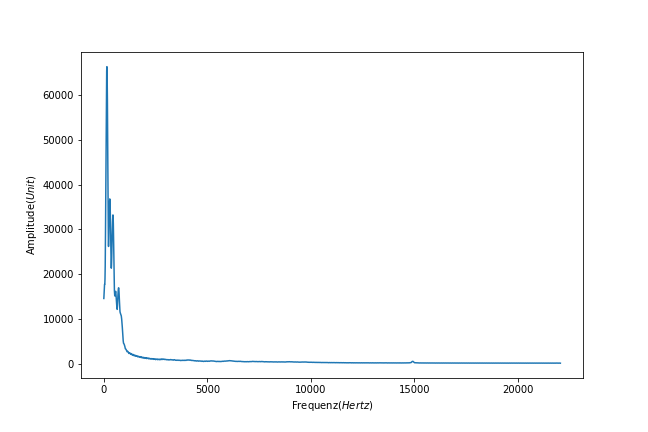
\includegraphics[width=12cm]{spektrum_mittel_windowshoch.png}
	\caption{Referenzspektrum von dem Befehl "Hoch"}
\end{figure}

\section{Messwerte}
\label{chap:VERSUCH_2_MESSWERTE}


\begin{table}[H]
\centering
\begin{tabular}{|l|l|l|1|}
\hline
\multicolumn{1}{|c|}{Spannung in V} & \multicolumn{1}{c|}{AD-Wandler}	& \multicolumn{1}{c|}{Philips}	& \multicolumn{1}{c|}{Keithley}								\\ \hline
1						&$1,035156250$		&$1,09$			&$1,039$ 		\\ \hline
2						&$1,992187500$		&$2$			&$2,001$		\\ \hline
3						&$3,007812500$		&$3,08$			&$3,06$			\\ \hline
4						&$4,062500000$		&$4,09$			&$4,07$			\\ \hline
5						&$5,078125000$		&$5,09$			&$5,082$		\\ \hline
6						&$5,986328125$		&$6,05$			&$5,998$		\\ \hline
7						&$7,050781250$		&$7,06$			&$7,01$			\\ \hline
8						&$8,066406250$		&$8,08$			&$8,022$		\\ \hline
9						&$9,082031250$		&$9,09$			&$8,986$		\\ \hline
10						&$9,980468750$		&$9,69$			&$9,999$		\\ \hline

\end{tabular}
\caption{Messwerte}
\end{table}
\section{Auswertung}

\label{chap:VERSUCH_2_AUSWERTUNG}

\textit{Korrelationskoeffizient nach Bravais-Pearson:} $$r_{fg}=\frac{\sigma_{fg}}{\sigma_{f}\cdot\sigma_{g}}$$ indem $\sigma_{f}$ und $\sigma_{g}$ jeweils Standardabweichungen von den entsprechenden Signalen f und g sind, die nach der Formel berechnet: $$\sigma^2_f=\frac{1}{n-1}\sum_{k=1}^{n}(f_k-\mu_f)^2$$
\qquad\textit{Die Kovarianz} $\sigma_{fg}$ ist für diskrete Signale definiert als:$$\sigma_{fg}=\frac{1}{n}\sum_{k=1}^{n}(f_k-\mu_f)\cdot(g_k-\mu_g)$$
\qquad $\mu_f$ ist \textit{der Mittelwert:} $$\mu_f=\frac{1}{n}\sum_{k=1}^nf_k$$

\begin{table}[H]
\centering
\begin{tabular}{|l|l|l|}
\hline
\multicolumn{1}{|c|}{Befehl} & \multicolumn{1}{c|}{Sprecher 1}		& \multicolumn{1}{c|}{Sprecher 2}			\\ \hline
Hoch						&$100\%$				&$100\%$				\\ \hline
Tief						&$100\%$				&$80\%$					\\ \hline
Links						&$100\%$				&$100\%$				\\ \hline
Rechts						&$100\%$				&$80\%$					\\ \hline
\end{tabular}
\caption{Detektionsrate}
\end{table}



Den Code davon bitte den Anhang A.1.3 und A.1.4 sehen.

\section{Interpretation}
\label{chap:VERSUCH_2_INTERPRETATION}
\qquad Die Detektion besagt, dass beim Sprecher 1 100$\%$ das Wort korrekt erkannt wurde und beim Sprecher 2 ist abweichend bei der Erkennung der Befehle "Tief$"$ und "Rechts". Das ist total verständlich, weil der Sprecher 1 ist die Person, von der die Referenzspektren hergestellt wurden. Bei dem anderen Sprecher wurde die Befehlen manchmal falsch erkannt. Die Erklärung dafür ist aus den anatomischen Gründe, dass jede Person eigene Stimme und eigene Sprechweise(Akzent) hat. Die Fehlerrate ist nicht so hoch, da die Datenbank der Referenzspektrum noch ziemlich klein ist (von nur 4 Befehlen).

%
% CHAPTER Anhang
%
\renewcommand\thesection{A.\arabic{section}}
\renewcommand\thesubsection{\thesection.\arabic{subsection}}

\chapter*{Anhang}
\label{chap:APPENDIX}
\addcontentsline{toc}{chapter}{Anhang}
%\setcounter{chapter}{0}
\addtocounter{chapter}{1}
\setcounter{section}{0}

\section{Quellcode}
\label{chap:APPENDIX_SOURCECODE}

\subsection{Quellcode Signal Aufnehmen, Triggerfunktion und Fourriertransformation}
\label{chap:APPENDIX_SOURCECODE_V1}
\begin{lstlisting}[
style=PYTHON,
frame=single,
caption=,
captionpos=b,
label=lst:V1]
import pyaudio 
import numpy as np
import matplotlib.pyplot as plt

FORMAT = pyaudio.paInt16
SAMPLEFREQ = 44100
FRAMESIZE = 1024
NOFFRAMES = 220
INPUT_BLOCK_TIME = 0.05 
INPUT_FRAMES_PER_BLOCK = int(SAMPLEFREQ*INPUT_BLOCK_TIME)
p = pyaudio.PyAudio()
print('running')
stream = p.open(format=FORMAT,channels=1,rate=SAMPLEFREQ, input=True,frames_per_buffer=FRAMESIZE)
data = stream.read(NOFFRAMES*FRAMESIZE) 
decoded = np.fromstring(data, 'Int16')
stream.stop_stream() 
stream.close() 
p.terminate() 
print('done') 

#######Signal speichern und darstellen########
string = 'hoch1'
np.save(string,decoded)
sec = len(decoded) / SAMPLEFREQ
plt.xlabel('Zeit in s')
plt.ylabel('Amplitude')
Zeit = []
for i in range (len(decoded)):
    Zeit.append(sec/len(decoded) * i)
plt.plot(Zeit,decoded) 
plt.show()

####Signal mit Triggerfunktion abschneiden####
trigger = 0.1 * np.max(decoded)
j = 0
for i in decoded:
    j = j + 1
    if np.abs(i) > trigger:
        decoded = decoded[j:j+SAMPLEFREQ]
        break
np.save(string+'abgeschnitten',decoded)
plt.xlabel('Zeit in s')
plt.ylabel('Amplitude')
Zeit = []
for i in range (len(decoded)):
    Zeit.append(1/len(decoded) * i)
plt.plot(Zeit,decoded) 
plt.show()

###########Fourriertranformation###############
spek = abs(np.fft.fft(decoded))
plt.plot(spek)
plt.savefig('Amplitudenspektrum.png')
\end{lstlisting}

\subsection{Quellcode Windowing und Spektrum Versuch 1}
\label{chap:APPENDIX_SOURCECODE_V1}
\begin{lstlisting}[
style=PYTHON,
frame=single,
caption=,
captionpos=b,
label=lst:V2]
import numpy as np
import matplotlib.pyplot as plt

def fft(data,name):
    plt.figure(figsize=(9,6))
    Y = abs(np.fft.fft(data))
    Y = Y[range(int(len(Y)/2))]
    x = np.linspace(0,22050,22050,endpoint = True)
    plt.xlabel('Frequenz($Hertz$)')
    plt.ylabel('Amplitude($Unit$)')
    plt.plot(x,abs(Y))
    plt.savefig(str(name)+".png")
    plt.show()
    
def winspek(data,name):
    plt.figure(figsize=(9,6))
    plt.xlabel('Frequenz($Hertz$)')
    plt.ylabel('Amplitude($Unit$)')
    st = np.std(data)
    from scipy import signal
    gfen = signal.gaussian(512, std = st * 4)
    g = np.zeros(len(data))
    fft = np.zeros(len(data))
    x = np.linspace(0,22050,22050,endpoint = True)
    for i in range(0,len(data),256):
        if (i > len(data) - 512):
            gfen = signal.gaussian(len(data)-i, std = st * 4)
            g[i:] = data[i:] * gfen
            fft += abs(np.fft.fft(g))
            a = np.fft.fft(g)
            a = a[range(int(len(a)/2))]
            plt.plot(x,abs(a))
            break
        g[i:i+512] = data[i:i+512] * gfen
        fft += abs(np.fft.fft(g))
        a = np.fft.fft(g)
        a = a[range(int(len(a)/2))]
        plt.plot(x,abs(a))
        g = np.zeros(len(data))
    plt.savefig("spektrum_gesamter_windows"+str(name)+".png")
    plt.show()
    fft /= 171 #durch die Anzahl der Windows teilen
    fft = fft[range(int(len(fft)/2))]
    plt.figure(figsize=(9,6))
    plt.xlabel('Frequenz($Hertz$)')
    plt.ylabel('Amplitude($Unit$)')
    plt.plot(x,fft)
    plt.savefig("spektrum_mittel_windows"+str(name)+".png")
    return fft
    
data = np.load('was_cooles_abgeschnitten.npy')
plt.figure(figsize=(9,6))
plt.xlabel('Zeit in s')
plt.ylabel('Amplitude')
Zeit = []
for i in range (len(data)):
    Zeit.append(1/len(data) * i)
plt.plot(Zeit,data)
plt.savefig("v1_abgeschnitten.png")
plt.show()
fft(data,"Amplitudenspektrum")

winspek(data,"v1")
\end{lstlisting}

\subsection{Quellcode Windowing und Referenzspektrum Versuch 2}
\label{chap:APPENDIX_SOURCECODE_V2}
\begin{lstlisting}[
style=PYTHON,
frame=single,
caption=,
captionpos=b,
label=lst:V2]
import numpy as np
import matplotlib.pyplot as plt
from scipy import signal

def winspek(data):
    st = np.std(data)
    gfen = signal.gaussian(512, std = st * 4)
    g = np.zeros(len(data))
    fft = np.zeros(len(data))
    for i in range(0,len(data),256):
        if (i > len(data) - 512):
            break
        g[i:i+512] = data[i:i+512] * gfen
        fft += abs(np.fft.fft(g))
        a = np.fft.fft(g)
        a = a[range(int(len(a)/2))]
        g = np.zeros(len(data))
    
    fft /= 171 #durch die Anzahl der Windows teilen
    fft = fft[range(int(len(fft)/2))]
    return fft

data = np.load('hoch1abgeschnitten.npy')
mit =  np.zeros(int(len(data)/2))
a = ['hoch', 'tief', 'rechts', 'links']
for j in a:
    mit = 0
    for i in range(1,6):
        data = np.load(j + str(i) + 'abgeschnitten.npy')
        np.save('spek' + j + str(i),winspek(data))
        mit+=winspek(data)
    mit = mit/5
    np.save('ref' + j,mit)
    plt.figure(figsize=(9,6))
    plt.xlabel('Frequenz($Hertz$)')
    plt.ylabel('Amplitude($Unit$)')
    plt.plot(mit)
    plt.savefig("spektrum_mittel_windows" + j + ".png")
    plt.show()
\end{lstlisting}

\subsection{Quellcode Korrelation und Spracherkenner Versuch 2}
\label{chap:APPENDIX_SOURCECODE_V2}
\begin{lstlisting}[
style=PYTHON,
frame=single,
caption=,
captionpos=b,
label=lst:V2]
import numpy as np

refhoch = np.load('experiment 2a/refhoch.npy')
reftief = np.load('experiment 2a/reftief.npy')
refrechts = np.load('experiment 2a/refrechts.npy')
reflinks = np.load('experiment 2a/reflinks.npy')
def spracherkenner(name,person):
    for i in range(1,6):
        test = np.load('Spek/spek'+str(name)+str(i)+'t'+str(person)+'.npy')
        korrcoefh = np.corrcoef(refhoch, y = test)
        korrcoeft = np.corrcoef(reftief, y = test)
        korrcoefr = np.corrcoef(refrechts, y = test)
        korrcoefl = np.corrcoef(reflinks, y = test)
        a = np.max([np.mean(korrcoefh), np.mean(korrcoeft), np.mean(korrcoefr), np.mean(korrcoefl)])
        if a == np.mean(korrcoefh):
            print('hoch')
        elif a == np.mean(korrcoeft):
            print('tief')
        elif a == np.mean(korrcoefr):
            print('rechts')
        elif a == np.mean(korrcoefl):
            print('links')
            
spracherkenner('links','p')
print("----")
spracherkenner('links','s')
\end{lstlisting}

\end{document}
%------------------------------------
% ╔═╗╔╗╔╔╦╗  ╔╦╗╔═╗╔═╗╦  ╦╔╦╗╔═╗╔╗╔╔╦╗
% ║╣  ║║║  ║║     ║║║  ║║    ║  ║║║║║ ╣  ║║║ ║ 
% ╚═╝╝╚╝═╩╝  ═╩╝╚═╝╚═╝╚═╝╩  ╩╚═╝╝╚╝  ╩ 
%------------------------------------